%-------------------------------------------------------------------------------
% LATEX TEMPLATE ARTIKEL
%-------------------------------------------------------------------------------
% Dit template is voor gebruik door studenten van de de bacheloropleiding 
% Informatica van de Universiteit van Amsterdam.
% Voor informatie over schrijfvaardigheden, zie 
%                               https://practicumav.nl/schrijven/index.html
%
%-------------------------------------------------------------------------------
%	PACKAGES EN DOCUMENT CONFIGURATIE
%-------------------------------------------------------------------------------

\documentclass{uva-inf-article}
\usepackage[english]{babel}
\usepackage{tikz}
\usepackage{pdflscape}
\usepackage{todonotes}
\usepackage{listings}
\usepackage[demo]{graphicx}
\usepackage{subcaption}
\lstset{
basicstyle=\small\ttfamily,
columns=flexible,
breaklines=true
}

\usepackage[style=authoryear-comp]{biblatex}
\addbibresource{references.bib}

%-------------------------------------------------------------------------------
%	GEGEVENS VOOR IN DE TITEL, HEADER EN FOOTER
%-------------------------------------------------------------------------------

% Geef je artikel een logische titel die de inhoud dekt.
\title{Shogun Post Documentation}

% Vul de naam van de opdracht in zoals gegeven door de docent en het type 
% opdracht, bijvoorbeeld 'technisch rapport' of 'essay'.
% \assignment{}
% \assignmenttype{}

% Vul de volledige namen van alle auteurs in en de corresponderende UvAnetID's.
\authors{Jari Andersen}
% \uvanetids{}

% Vul de naam van je tutor, begeleider (mentor), of docent / vakcoördinator in.
% Vermeld in ieder geval de naam van diegene die het artikel nakijkt!
% \tutor{}
% \mentor{}
% \docent{}

% Vul hier de naam van je tutorgroep, werkgroep, of practicumgroep in.
% \group{SignLab, VisualisationLab}

% Vul de naam van de cursus in en de cursuscode, te vinden op o.a. DataNose.
% \course{}
% \courseid{}

% Dit is de datum die op het document komt te staan. Standaard is dat vandaag.
\date{\today}

%-------------------------------------------------------------------------------
%	VOORPAGINA 
%-------------------------------------------------------------------------------

\begin{document}
\maketitle

%-------------------------------------------------------------------------------
%	INHOUDSOPGAVE EN ABSTRACT
%-------------------------------------------------------------------------------
% Niet toevoegen bij een kort artikel, zeg minder dan 10 pagina's!

%TC:ignore
\tableofcontents
%\begin{abstract}
%\end{abstract}
%TC:endignore
\newpage
%-------------------------------------------------------------------------------
%	INHOUD
%-------------------------------------------------------------------------------
% Hanteer bij benadering IMRAD: Introduction, Method, Results, Discussion.
\section{Introduction}
Welcome to the Shogun Post Documentation! In this guide, we delve into various tools and skills within Shogun Post, designed to streamline your post-production workflows effectively. Throughout this documentation, we'll address crucial aspects such as identifying and resolving bugs, as well as highlighting best practices to optimize your post-production processes. Additionally, we'll delve into scripting techniques and the creation of efficient export pipelines, empowering you to automate tasks and enhance productivity.
Our exploration extends to a range of indispensable tools, including retargeting mechanisms, strategies for rectifying marker issues, and integration techniques for importing StretchSense data.

\section{Best practices and tips}
This section will go over various best practices and tips to help aid in the process of post processing within Shogun Post.

\subsection{Fixing marker data}
When recording motion capture data, a lot can go wrong. Markers aren't always tracked perfectly and the cameras/system will make wrong assumptions in regards to the markers. Markers can become occluded, missed, or mistaken for different markers. They may not be tracked optimally, resulting in jittery data, and sometimes the cameras may even detect markers that are not present in reality. Some of these issues are fixable in Shogun Post. This section goes over these issues and explains how these are fixed.

In Post, we have the ability to:
\begin{itemize}
    \item Reconstruct dropped frames
    \item Review the data health
    \item Label markers\\Tell the system which markers are supposed to be which. The labeling process can also include un-labeling markers.
    \item Filtering marker recordings\\Over a recording period, we can filter marker recordings. This can result in less jittery marker data.
    \item Fix missing markers
    \item Apply the changes to the animation data.
\end{itemize}

In the following subsub-sections we will go over these techniques in order on how you would apply them in Shogun Post. For the sake of fixing marker data, I recommend using the labeling view filters preset for the 3D View Filters (figure \ref{fig:viewfilters}). Lastly, it is important to note that through experience I've found that it is not always necessary to fix all issues relating to marker data. Look at the resulting animation and make a decision based on what you see. If there is nothing weird going on. Than there is no need to fix everything.

\begin{figure}[hbt!]
    \centering
    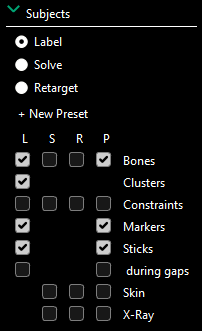
\includegraphics[width=0.1\textheight]{imgs/viewFilters.png}
    \caption{Shogun Post labeling preset for the 3D view filters.}
    \label{fig:viewfilters}
\end{figure}




\subsubsection{Reconstruct dropped frames}
When loading an .mcp file, and if frames are dropped during recording. In Shogun Post we can either use a simple interpolation over these frames, or ask Post to reconstruct the data based on the raw 2D data of the cameras. On import of an .mcp we get prompted by Post if we want this (figure \ref{fig:dropfix}). My recommendation is to use the latter option.
\begin{figure}[hbt!]
    \centering
    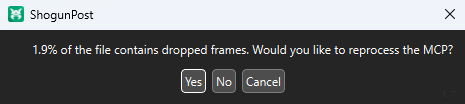
\includegraphics[width=0.5\textwidth]{imgs/DataMgtDropFix.png}
    \caption{Shogun Post prompt on reprocessing the dropped frames.}
    \label{fig:dropfix}
\end{figure}

\subsubsection{Review the data health}
For the purpose of identifying where in the recording most problems lie, Shogun Post provides the ``issue map" (figure \ref{fig:shogunPostTimeline}). This issue map shows two horizontal bars in the timeline where the bars are colored yellow to red when issues are located. The more red the bar turns the more markers display issues. The top section indicates unlabeled markers, whilst the lower bar indicates solving constraints. We have the ability to double click on these issues, and Shogun Post will then zoom in on the markers that display the issue. In order to gain a better understanding of these problems, Shogun Post provides the ``Data Health view" (figure \ref{fig:datahealth}). It offers visual indicators and metrics to assess the health of the motion capture data, such as marker visibility, marker gaps, and frame rate consistency. By examining the gaps and outlined blocks in the data health view, we are able to spot problem areas more effectively.

\begin{figure}[hbt!]
    \centering
    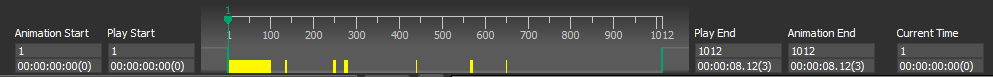
\includegraphics[width=1.\textwidth]{imgs/ShogunPostTimeline.png}
    \caption{Shogun Post's timeline. Left is ``Animation Start" and right is ``Animation End".}
    \label{fig:shogunPostTimeline}
\end{figure}

\begin{figure}[hbt!]
    \centering
    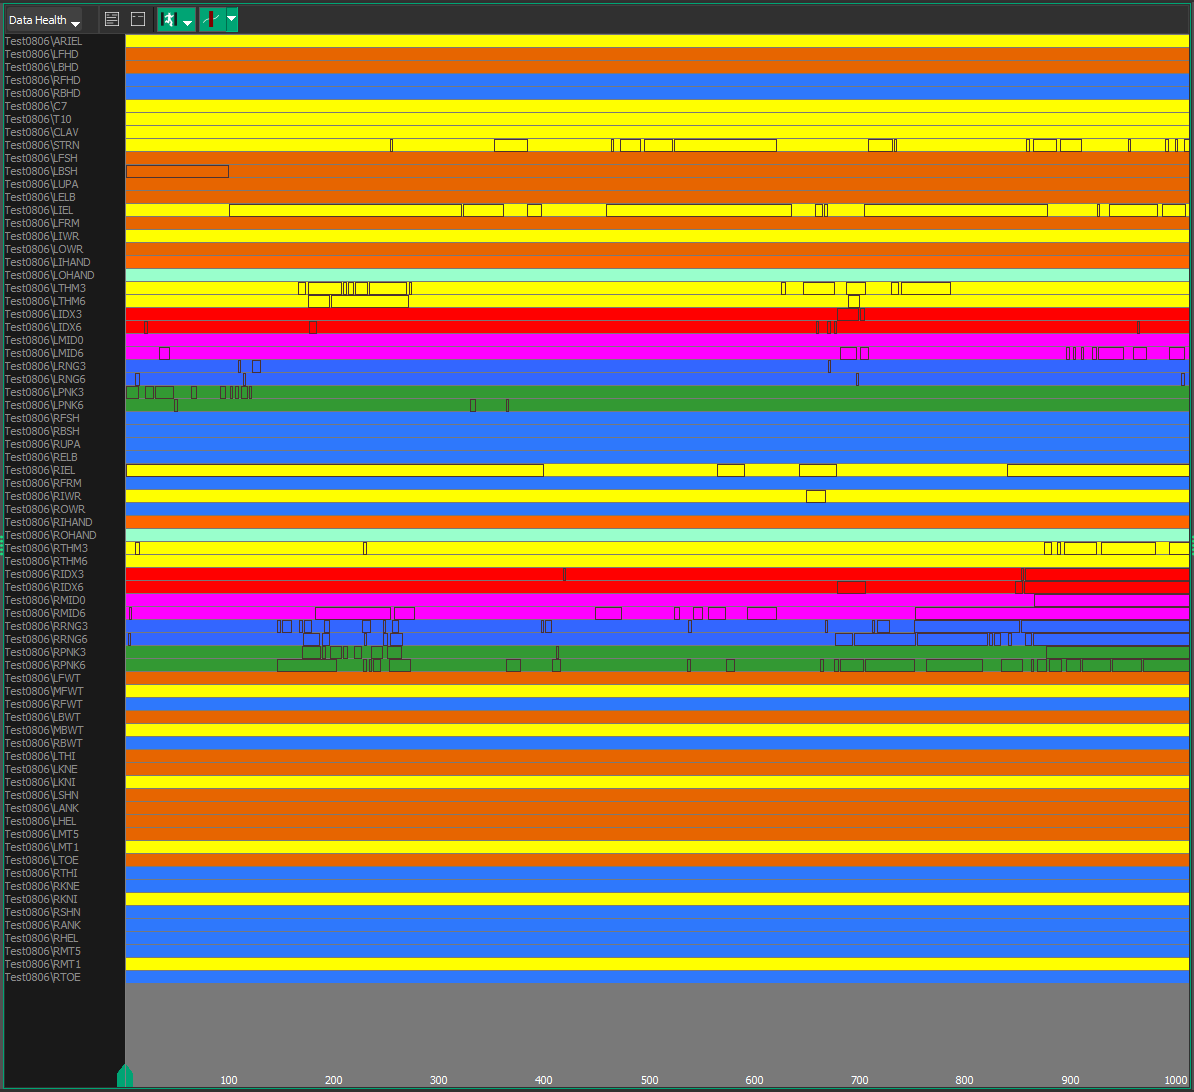
\includegraphics[width=.8\textwidth]{imgs/datahealth.png}
    \caption{Shogun Post's Data Health tab. Left are all the marker labels, and the colored scheme displays potential problem areas.}
    \label{fig:datahealth}
\end{figure}

\subsubsection{Labeling markers}
Vicon is a ``Passive marker-based motion capture system". What this entails is that the markers hold no identity themselves. The identity, in the form of labels, is given to them based on the constellation of neighbouring markers during recording. The markers are then used to create a skeleton. This process is called a solve. However, such a system has its disadvantages. During recording, markers can experience label errors when they are lost (for example, due to occlusion) or mistaken for other markers (a phenomenon known as swapping). Additionally, markers can sometimes appear in the recording even though they do not exist in real life, resulting in stolen labels. All of these issues can be solved in the labeling tab in Shogun Post (figure \ref{fig:labeling}). An example of the process of fixing labeling errors can be found in the following link: \url{https://www.youtube.com/watch?v=BBCqKjJ4ASc}. I highly recommend that you watch through the video, a visual example is more intuitive than a written explanation.

In the labeling tab, we have the ability to select a label and then a marker to assign the correct label (or vice versa if you enable ``select mode", see top right of figure \ref{fig:labeling}). We are able to assign these for the whole take, a specific frame, all regions within a specified gap size (cliffs), or a selected region. In the ``Manual Labeling Tools" section, we are able to correct swaps, and we can un-label.

The process of fixing the labels is relatively straightforward. We go through the entire take and we identify areas where the animation displays odd behavior due to labeling errors. The labeling tab displays errors in the current frame by highlighting labels in a color range from yellow through red, where yellow is a missed or missing label and red is a label missing entirely (meaning that we cannot find it in the scene). To correct a swap, select one of the swapped labels and then select the corresponding marker. This will un-label the other marker. To correct an un-labeled marker, select the label and the corresponding marker. \textit{Note: if you have select mode enabled, you select the marker in the scene first and then the marker in the labelling-tab.}

\begin{figure}[hbt!]
    \centering
    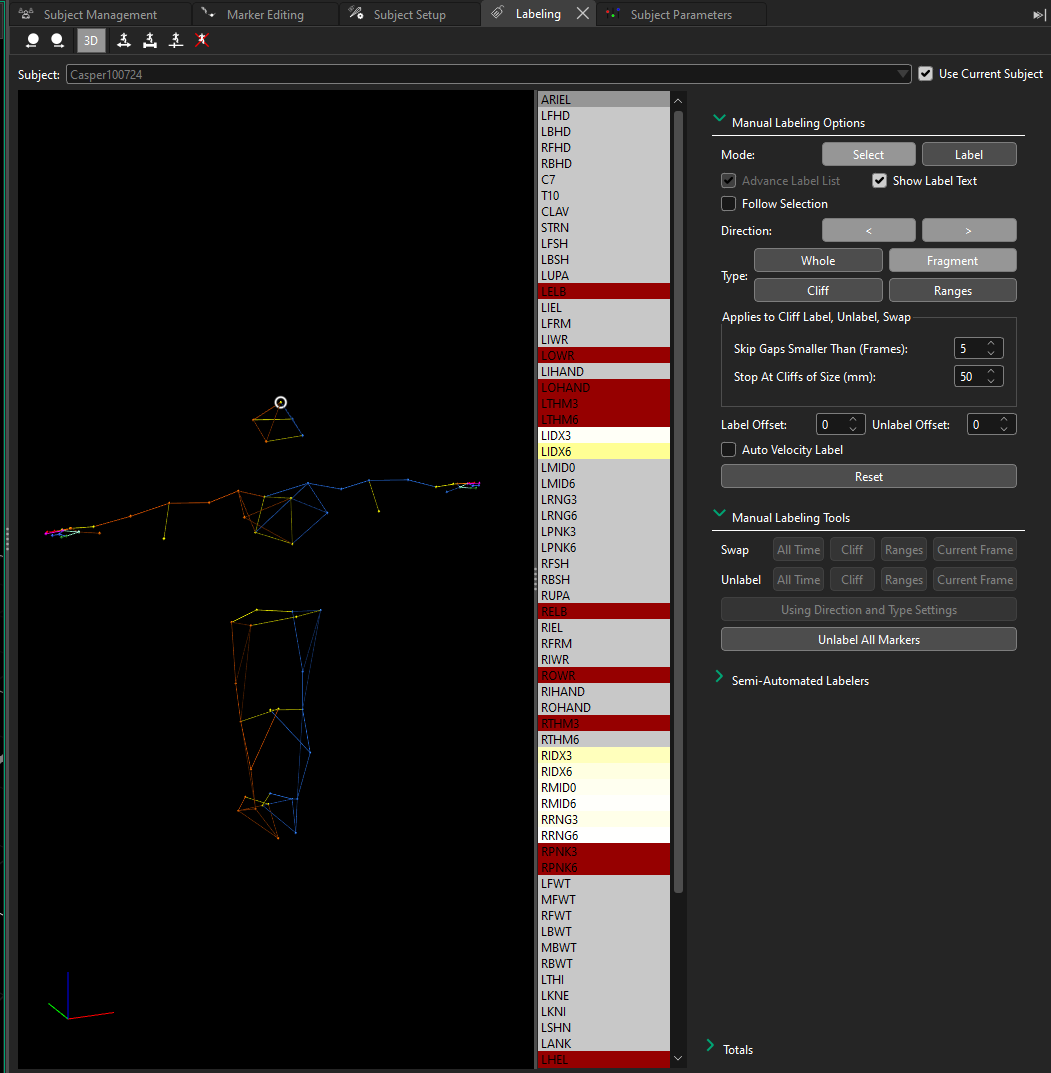
\includegraphics[width=.8\textwidth]{imgs/labeling.png}
    \caption{Shogun Post's Data Health tab. Left are all the marker labels, and the colored scheme displays potential problem areas.}
    \label{fig:labeling}
\end{figure}

\subsubsection{Missing markers and jittering markers}
A marker can be completely out of sight of each camera, resulting in a missing marker. Vicon attempts to predict where a missing marker is located and apply this to the recording. A missing marker will appear in the scene as a red light (figure \ref{fig:missingmarker}). An example of the process of fixing missing markers and jittering markers can be found in the following link: \url{https://www.youtube.com/watch?v=ZoYldRNvWuc}. Again, I highly recommend that you watch through the video, a visual example is more intuitive than a written explanation.

\begin{figure}[hbt!]
    \centering
    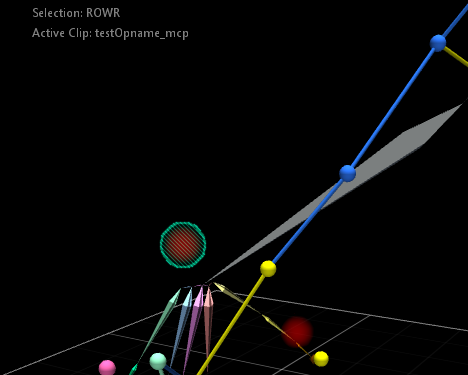
\includegraphics[width=.8\textwidth]{imgs/missingMarker.png}
    \caption{A missing marker labeled as ROWR (right outside wrist).}
    \label{fig:missingmarker}
\end{figure}

After a missing marker is labeled (either by manually or already by Shogun), we can use the techniques in the ``marker editing tab" to decide how we want to fill in this data. The following options are for filling in missing gaps. We pick based on the type of issue we have:
\begin{itemize}
    \item Interpolation\\
    With the interpolation method we can fill in gaps by interpolating between the beginning and end of the problem area. This is used when we are simply missing a marker that doesn't rely on neighbouring markers and when the motion is fairly linear.
    \item Rigid\\
    With the rigid method we can specify neighbouring markers of the missing marker. When we do this, Shogun Post will constrain the marker position based on its neighbours when filling the gap by using the trajectory data of the neighbours. This is especially useful for markers that stay in the same position relative to a set of other markers (for example the six markers placed around the waist area of the actor).
    \item Constraint\\
    The constraint method is our only method we can use when the movement is non linear, and we aren't able to rigid fill because all the neighbouring markers that display the same trajectory are missing. This method uses the solved animation to fill in the missing markers. By inspecting the missing markers during the gap, and validating whether the motion is correct during the gap, we are able to judge if this method will work.
\end{itemize}

The marker editing tab also allows us to edit jittering markers. After selecting the problematic range in the graph view, we go to the ``Default Filters" section where we can choose between heavy, medium, light, and very light filtering to fix the jittering. One of the advantages of this filtering, is that it is additive. Meaning that we can select an option multiple times to filter the jittering out little by little. In addition, we can setup custom filters.

\subsubsection{Applying the fixes}\label{sec:applyFix}
It is important to note that after editing a marker or label, that we want to apply the changes on the animation. Not only for the eventual export, but applying in between fixing markers can help with visualising the issue. To apply the changes onto the skeletal-animation data we recalculate the solve in the processing tab.

\subsection{Solving constraints: the r-handform}
In our quest to animate complex handforms, such as the r-handform. We have one very strong weapon: solving constraints. When viewing figure \ref{fig:originalR:sfig2}, we can see how Vicon has successfully tracked the markers for the r handform. The red markers (index finger) are underneath and crossed with the purple markers (middle finger). Even though this was successful, the avatar is not displaying an accurate r-handform (see figure \ref{fig:originalR:sfig1}). Luckily, we can tell Vicon's solver to follow the constraints related to these fingers more closely. Go to the subject setup tab $>$ solving $>$ modify setup $>$ Constraints in Current Subject location. Here we can alter the following five positional constraints:
\begin{itemize}
    \item RightHandIndex\_RMCP22
    \item RightHandIndex2\_RIDXM2
    \item RightHandIndex3\_RIDXD2
    \item RightHandMiddle1\_RMFRP2
    \item RightHandMiddle3\_RMFRD2
\end{itemize}
Set these to a weight above 4 for the best results (feel free to play around with adding other positional constraints and altering the weight). When prompted with ``The solving subject contains expressions which prevent hand editing. Would you like to remove all solving parameterization from this subject?", select ``No". Lastly, just like in section \ref{sec:applyFix}, we have to apply the changes by solve solving in the processing tab. When the solver is done we can enjoy our results for the r-handform (see figure \ref{fig:comparisonR} for a before and after).

Lastly, in order to avoid having to do this for every take, we export the altered solving skeleton and use that for our recordings in Shogun Live (see \url{https://youtu.be/j1-_MGfP_zE?t=125&si=mhbs0C4o8prmcD2f} on how to achieve this).

\begin{figure}[hbt!]
\begin{subfigure}{.5\textwidth}
  \centering
  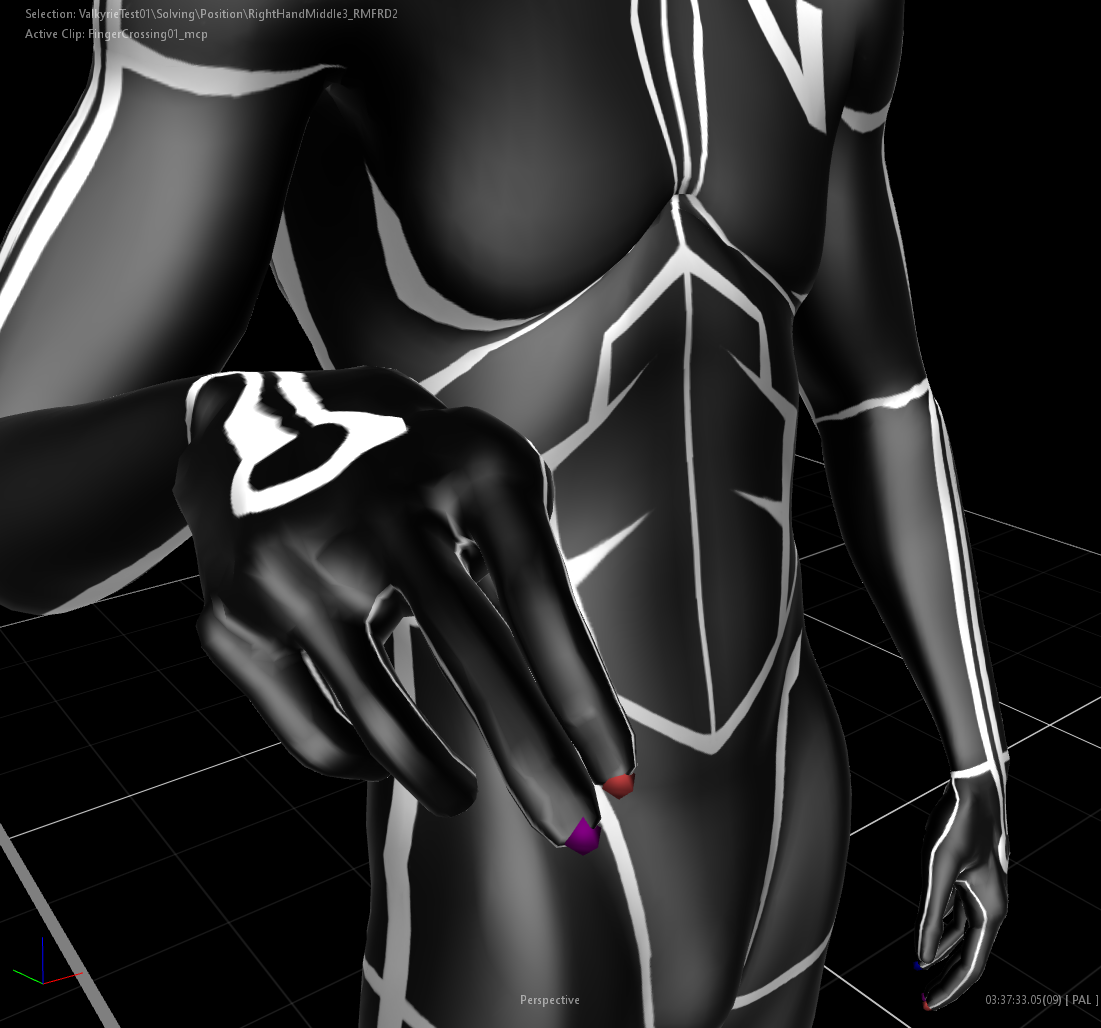
\includegraphics[width=.8\linewidth]{imgs/r-handform/noR.png}
  \caption{The original solve with no alterations for the r-handform.}
  \label{fig:originalR:sfig1}
\end{subfigure}%
\begin{subfigure}{.5\textwidth}
  \centering
  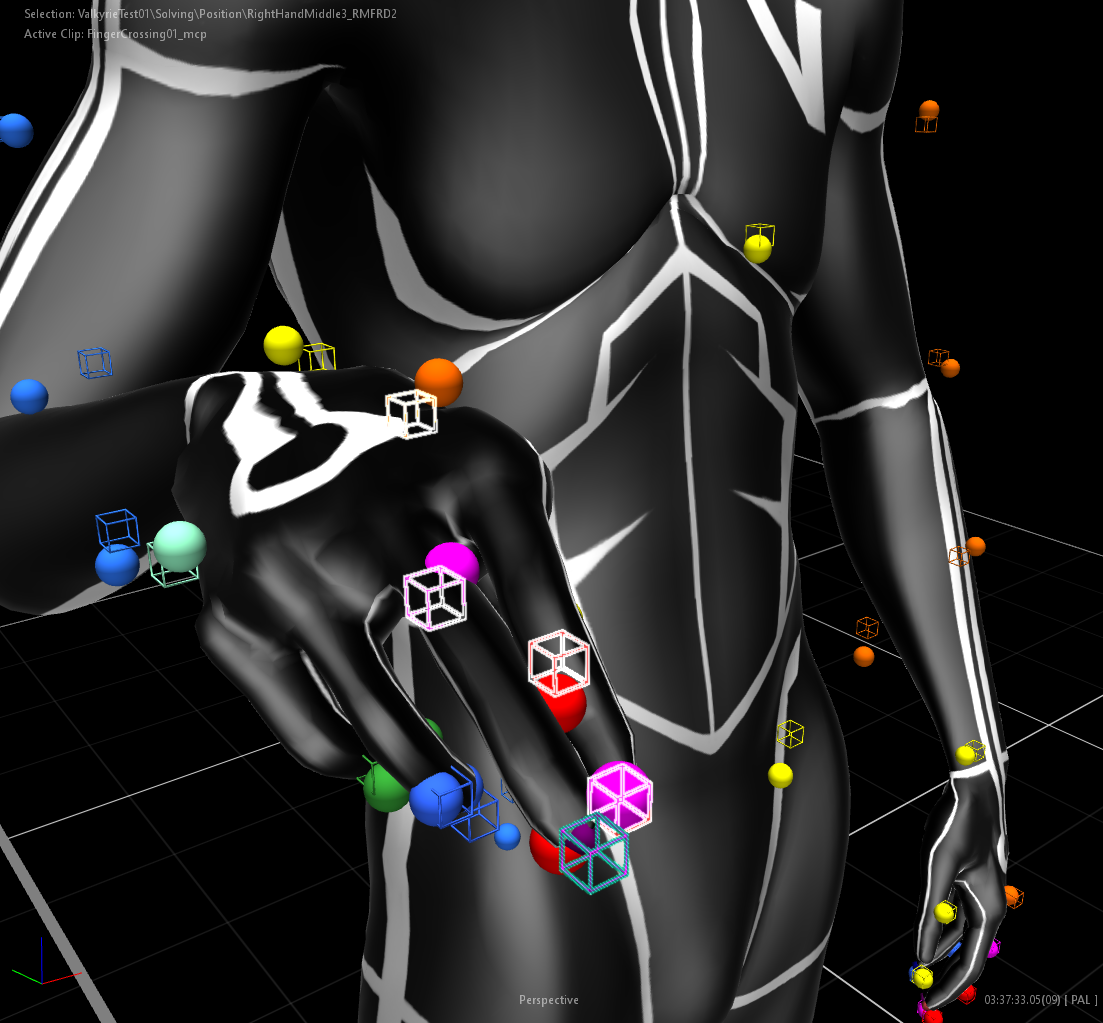
\includegraphics[width=.8\linewidth]{imgs/r-handform/constraintsR.png}
  \caption{The solving constraints (highlighted) which can be used to improve the r-handform.}
  \label{fig:originalR:sfig2}
\end{subfigure}
\caption{The original solve and constraints. We can see how there are discrepancies on where the markers are placed and how the hand is solved.}
\label{fig:originalR}
\end{figure}

\begin{figure}[hbt!]
\begin{subfigure}{.5\textwidth}
  \centering
  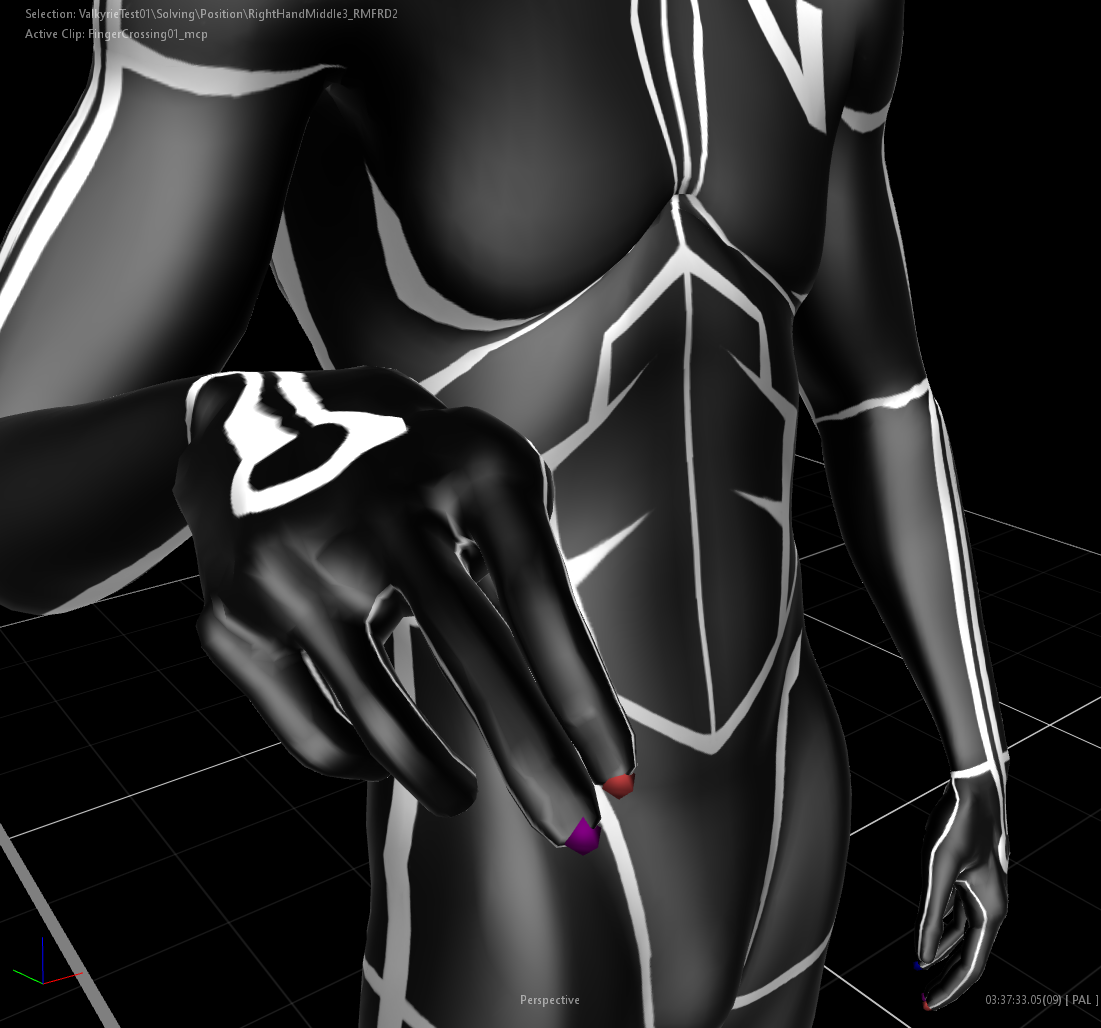
\includegraphics[width=.8\linewidth]{imgs/r-handform/noR.png}
  \caption{The original solve with no alterations for the r-handform.}
  \label{fig:comparisonR:sfig1}
\end{subfigure}%
\begin{subfigure}{.5\textwidth}
  \centering
  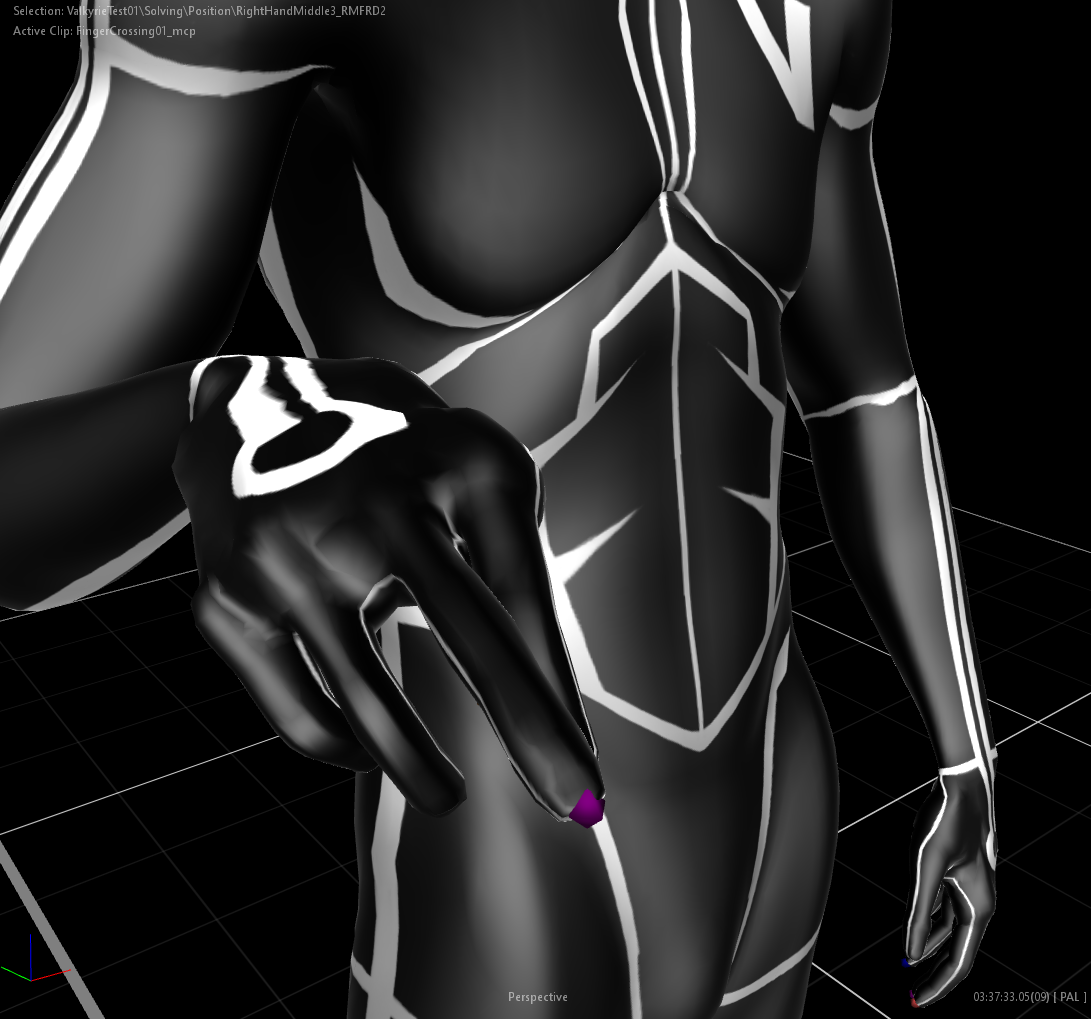
\includegraphics[width=.8\linewidth]{imgs/r-handform/finalR.png}
  \caption{The resulting r-handform, after applying higher weights to the related solving constraints.}
  \label{fig:comparisonR:sfig2}
\end{subfigure}
\caption{The original results for the r-handform (left) versus the altered results (right).}
\label{fig:comparisonR}
\end{figure}

\subsection{Retargeting}
\todo{Process in short, tips on hands}

\subsection{Creating scripts}
Creating Scripts in Shogun Post can be done through their script editor. Here are some more tips on them:
\begin{itemize}
    \item Use scripts by Vicon from the script folder to get an idea on how to write them.
    \item Use the record function in Shogun Post's script editor to record your clicks and actions in the software (see Figure \ref{fig:recordButton}). This will make finding certain functionalities and scripting quickly much easier.
    \item If you want to reuse scripts, make buttons for them by right clicking somewhere in the upper tab. You can also create new tabs for buttons.
\end{itemize}

\begin{figure}[hbt!]
    \centering
    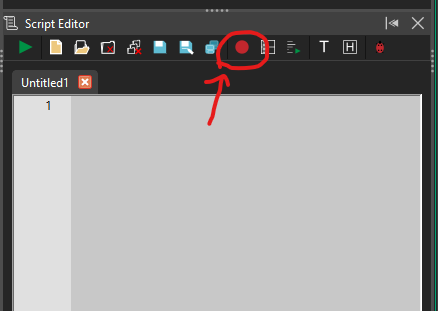
\includegraphics[]{imgs/recordButton.png}
    \caption{Location of the scripting record button in Shogun Post.}
    \label{fig:recordButton}
\end{figure}


\subsection{Export pipelines}
Often, when recording many takes, we want to export each of them out of Shogun Post in the same manner. For this, we can use the ``Batching" functionalities (see Figure \ref{fig:batching}). In the Batching tab, we can select which files we want to export, and define where and how they should be exported. 
\begin{figure}[hbt!]
    \centering
    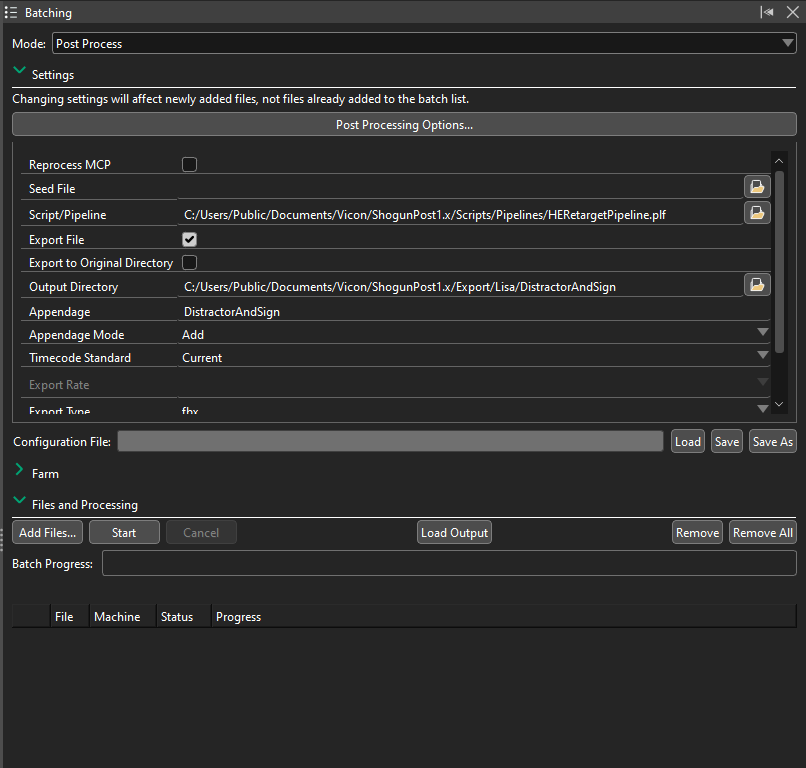
\includegraphics[width=\textwidth]{imgs/Batching.png}
    \caption{The batching tab in Shogun Post.}
    \label{fig:batching}
\end{figure}

These functionalities however, are not always enough. For example, if we want to remove the ``wand" prop from every take, we would not be able to do this with the default functionalities. To this end, we can create pipeline scripts (extension ``.plf"). In the pipeline scripts we can define what operations (hsl or py scripts) to run before exporting a take. See Figure \ref{fig:pipelineHE} for an example pipeline that sets a frame rate, imports StretchSense FBX files and retargets before exporting.
\begin{figure}[hbt!]
    \centering
    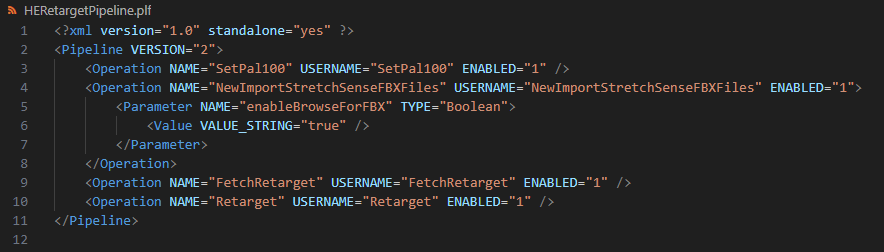
\includegraphics[width=\textwidth]{imgs/pipelineHE.png}
    \caption{An example pipeline script where we want to set the frame rate to PAL100, import StretchSense fbx files, and retarget before exporting.}
    \label{fig:pipelineHE}
\end{figure}


\subsection{Combining Vicon and StretchSense data}
We follow the guide in the following link: \url{https://www.youtube.com/watch?v=6kPKS7FgRa0}. Important to note is, after importing the hands, the mesh from Vicon breaks. The skeleton will only be useful for retargeting from there on out. In addition we note the following tips:
\begin{itemize}
    \item If the auto-align fails for the retargeted skeleton, use that functionality before importing the StretchSense hands.
    \item Make sure to only use rotation constraints for the fingers.
    \item Pose the hands of the source and target skeleton in the same manner.
\end{itemize}


\section{Bugs and fixes}
In this section we go over various bugs we found and fixes to solve them.

\subsection{Unreal import / no animation bug}
\begin{figure}[hbt!]
    \centering
    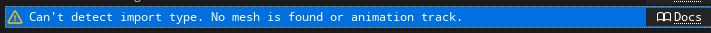
\includegraphics[width=\textwidth]{imgs/UEImportBug.png}
    \caption{Unreal import bug.}
    \label{fig:importBugUE}
\end{figure}
When importing a retarget into Unreal Engine, we came acros the following bug: ``Can't detect import type. No mesh is found or animation track". In Shogun Post everything seems to be working, the retargeted animation is displayed and we selected the retarget branch for export. Although no errors were recorded in Shogun Post, the bug is attributed to issues within the software itself. After importing the retargeted FBX animations into Blender, we can view the skeleton, but the animation itself is not present. In our case, the bug occurred because we altered the frame rate after retargeting. To fix this, simply retarget over the playrange again and export like usual. I believe the displayed animation appears correct after altering the frame rate because it is consistently interpolated between frames.


%-------------------------------------------------------------------------------
%	REFERENTIES
%-------------------------------------------------------------------------------

\printbibliography

%-------------------------------------------------------------------------------
%	BIJLAGEN 
%-------------------------------------------------------------------------------

%TC:ignore
% \appendix 
% \section{Bijlage {\LaTeX} code}
% Bijgevoegd zijn de \textattachfile{main.tex}{code} en 
% \textattachfile{references.bib}{bibliografie}.
%TC:endignore

%-------------------------------------------------------------------------------
\end{document}